%%%%%%%%%%%%%%%%%%%%%%%%%%%%%%%%%%%%%%%%%
% Beamer Presentation
% LaTeX Template
% Version 1.0 (10/11/12)
%
% This template has been downloaded from:
% http://www.LaTeXTemplates.com
%
% License:
% CC BY-NC-SA 3.0 (http://creativecommons.org/licenses/by-nc-sa/3.0/)
%
%%%%%%%%%%%%%%%%%%%%%%%%%%%%%%%%%%%%%%%%%


\documentclass{beamer}

\mode<presentation> {

%\usetheme{default}
\usetheme{Boadilla}
%\usetheme{CambridgeUS}
%\usetheme{Madrid}

  \usefonttheme{default}  % or try serif, structurebold, ...
  \setbeamertemplate{navigation symbols}{}
  \setbeamertemplate{caption}[numbered]
}

\definecolor{darkblue}{rgb}{0,0,0.8}
\definecolor{darkgreen}{RGB}{78,104,81}
\definecolor{lightgreen}{RGB}{130,173,135}
\definecolor{lightgray}{RGB}{122, 122, 122}
\setbeamercolor{palette primary}{bg=darkgreen,fg=white}
\setbeamercolor{palette secondary}{bg=lightgreen,fg=white}
\setbeamercolor{palette tertiary}{bg=darkgreen,fg=white}
%\setbeamercolor{palette quaternary}{bg=wolfred,fg=white}
\setbeamercolor{structure}{fg=black} % itemize, enumerate, etc
\setbeamercolor{frametitle}{bg=white}

%\usepackage{tikz,pgfpages}
%\usetikzlibrary{shapes,arrows,trees,mindmap,decorations.pathreplacing}

\usepackage{graphicx} % Allows including images
\usepackage{booktabs} % Allows the use of \toprule, \midrule and \bottomrule in tables
\usepackage{multicol}

\setbeamercolor{block title}{use=structure,fg=structure.fg,bg=structure.fg!20!bg}
\setbeamercolor{block body}{parent=normal text,use=block title,bg=block title.bg!50!bg}

\definecolor{Mahogany}  {RGB}{20,50,100}


\usepackage{colortbl}

\usepackage{algorithm,algorithmic,color}

\newcommand{\black}[1]{{\color{black}{#1}} }
\newcommand{\green}[1]{{\color{green}{#1}} }
\newcommand{\blue}[1]{{\color{blue}{#1}} }
\newcommand{\red}[1]{{\color{red}{#1}} }
\newcommand{\vect}[1]{\boldsymbol{#1}}



\title[Hybrid Splicing]{Hybrid Splicing of Multi-Scale Downscaler Air Quality Surfaces} 

\author{Elizabeth Herman} 

\author[H, L, L, O, N, R, S ]{Elizabeth Herman, Jeonghwa Lee, Kartik Lovekar, Dorcas Ofori-Boateng, Fatemeh Norouzi, Benazir Rowe, and Jianhui Sun} 
\institute[IMSM 2018]{Industrial Math/Stat Modeling Workshop 2018}
\date{July 25, 2018} 

\begin{document}

\begin{frame}
\titlepage 
\end{frame}


%---------------------------------------------------
%   PRESENTATION SLIDES
%---------------------------------------------------

\begin{frame}{Motivation}

\begin{columns}
\begin{column}{4cm}
In 2016, 
\begin{itemize}
\item 122.5 million people live in countries high levels of air pollutant concentrations
\item 12.1 million people live in countries which have high levels of PM-25
\item 7 million people died from air pollutants
\end{itemize}

\end{column}
\begin{column}{7cm}
\vspace{-3mm}
%\\\hspace{10mm}\includegraphics[width=.35\textwidth]{ode35setup.pdf}\hspace{15mm}
\begin{center}
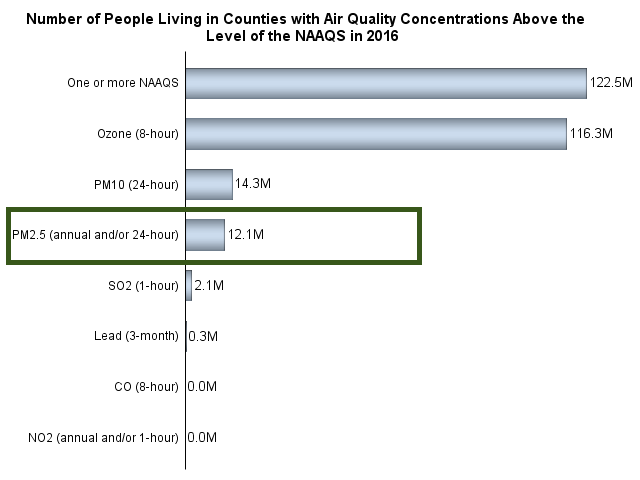
\includegraphics[width=1.0\textwidth]{pollution.png}
\end{center}

\end{column}
\end{columns}
\begin{center}
\small{\textcolor{lightgray}{http://www.who.int/gho/phe/air\_pollution\_mortality/en/}}
\\\small{\textcolor{lightgray}{https://www.epa.gov/air-trends/air-quality-national-summary}}
\end{center}
\end{frame}

\begin{frame}{Problem Set-up: Data of air pollution concentrations}
\begin{columns}
\begin{column}{6cm}
\vspace{-5mm}
\begin{itemize}
\item Air Quality System (AQS): Point-source measurements (usually near large cities)\vspace{3mm}
\item IMPROVE sites: Point-source measurements (usually near rural areas)\vspace{3mm}
\item Downscaler Model (DS): fuses estimates of pollutant obtained through a model that uses current knowledge of the atomshpere and AQS readings using a spatially-varying weighted model
\end{itemize}

\end{column}
\begin{column}{5cm}
\vspace{-5mm}
%\\\hspace{10mm}\includegraphics[width=.35\textwidth]{ode35setup.pdf}\hspace{15mm}
\begin{center}
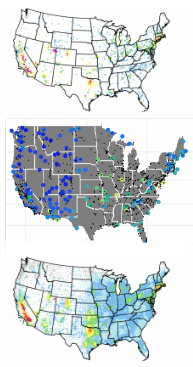
\includegraphics[width=0.85\textwidth]{DataSources.png}
\end{center}

\end{column}
\end{columns}

\end{frame}

\begin{frame}{Problem Set-up: Downscaler}
\textbf{Old method:} Run Downscaler on National surface
\begin{center}
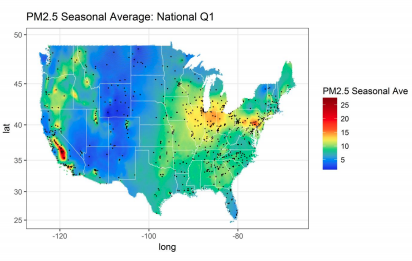
\includegraphics[width=0.6\textwidth]{NationalDS.png}
\end{center}

\textbf{New method:} Run Downscaler over regional surface
\begin{itemize}
\item In Downscaler, there is one range parameter
\item Run regions in parallel
\item Perform better
\end{itemize}


\end{frame}

\begin{frame}{Regions: Climate Zones}
\vspace{-5mm}
\begin{center}
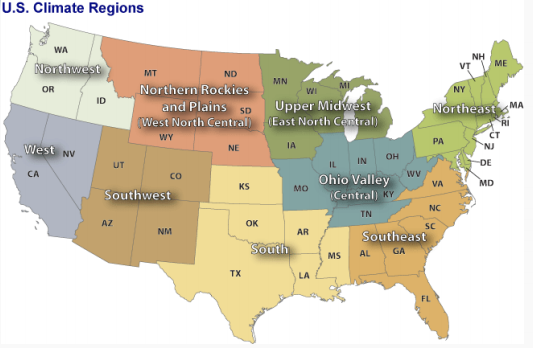
\includegraphics[width=1.0\textwidth]{ContUS.png}
\end{center}
\end{frame}

\begin{frame}{Regions: Downscaler}
\vspace{-5mm}
\begin{center}
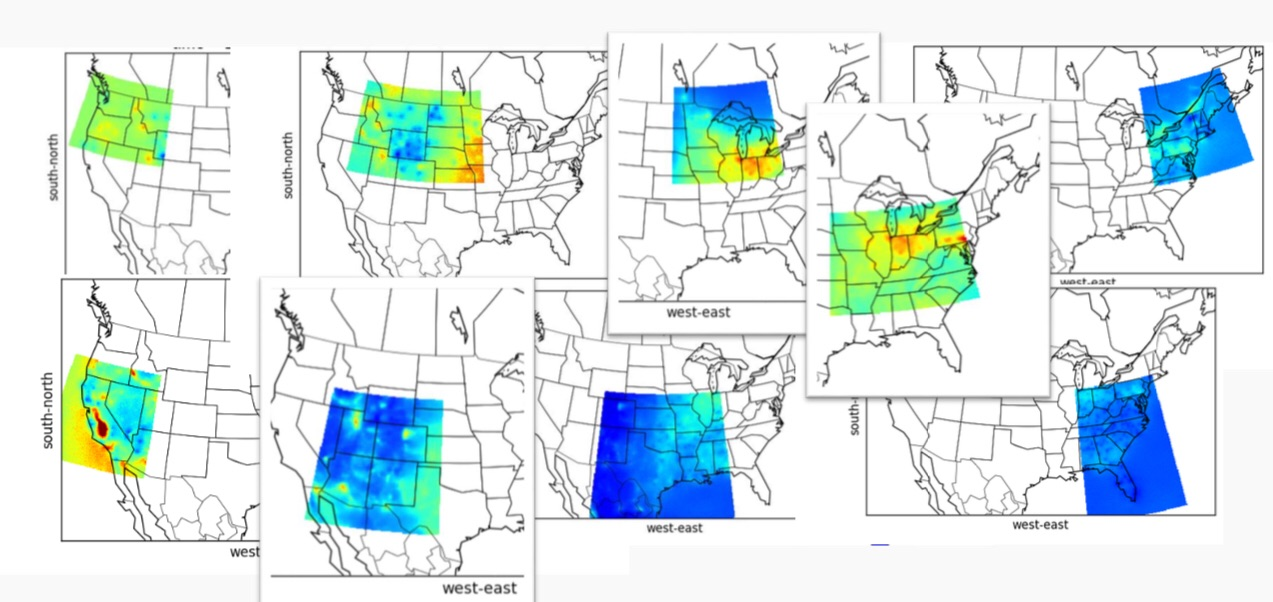
\includegraphics[width=1.0\textwidth]{RegionalDS.jpg}
\\
\vspace{3mm} Run the Downscaler on the NOAA climate regions with overlap area.
\\\vspace{3mm} \textbf{Question: How to deal with the multiple values in the overlap region?}
\end{center}

\end{frame}

\begin{frame}{Regions: Overlap}
\vspace{-3mm}
\begin{center}
\textbf{Question: How to deal with the multiple values in the overlap region?}
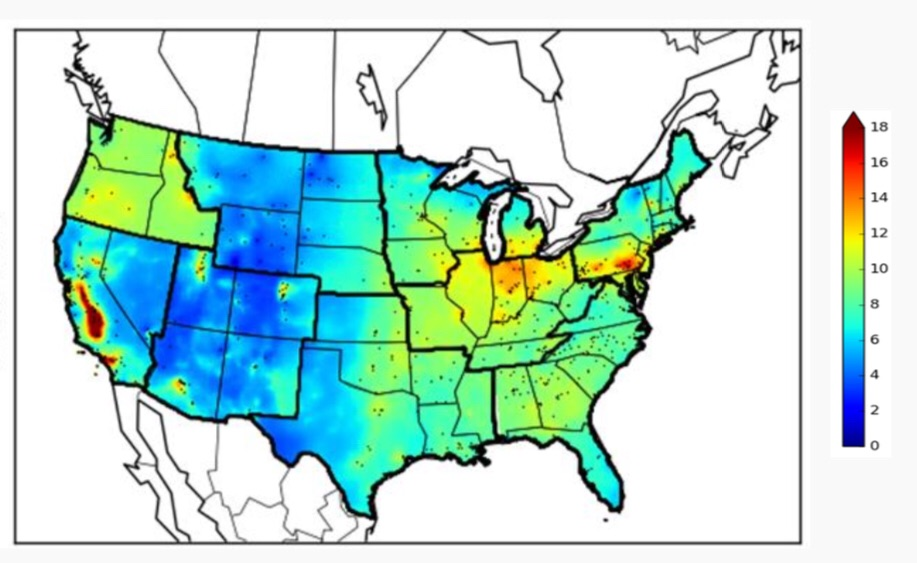
\includegraphics[width=0.9\textwidth]{patchwork.jpg}
\end{center}

\end{frame}

\begin{frame}{Assumptions}
\vspace{-5mm}
\begin{center}
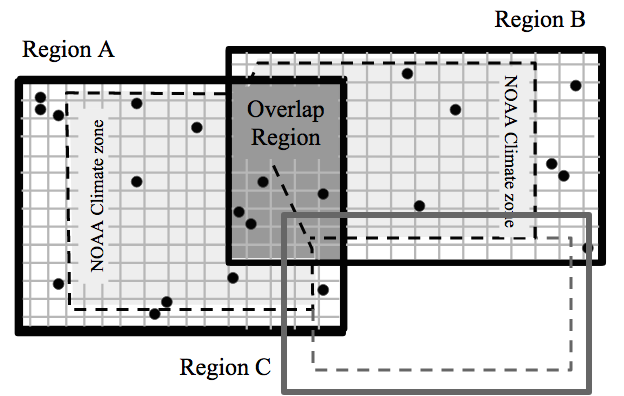
\includegraphics[width=1.0\textwidth]{overlap.png}
\end{center}
\end{frame}

\begin{frame}{Methodology}

\end{frame}

\begin{frame}{Methodology}

\end{frame}


\begin{frame}{Results}

\end{frame}

\begin{frame}{Results}

\end{frame}

\begin{frame}{Results}

\end{frame}

\begin{frame}{Statistics}

\end{frame}

\begin{frame}{Conclusion and Future Work}
\textbf{Conclusion:}
\begin{itemize}
\item Developed methodology to splice two region values together
\item Provided statistics to show our method is correct
\end{itemize}
\vspace{9mm}
\textbf{Future Work:}
\begin{itemize}
\item Working on multiple zones simultaneous
\item Incorporate longitude \textbf{AND} latitude distances
\end{itemize}

\end{frame}


\begin{frame}
\begin{center}\textbf{THANK YOU!}\end{center}
\begin{itemize}
\item Elisabeth Mannshardt, Barron Henderson, and Brett Gantt
\item Brian Reich
\item Organizers of IMSM
\item SAMSI
\end{itemize}

\vspace{7mm}
\begin{center}
\textbf{QUESTIONS}
\end{center}
\end{frame}

\begin{frame}{References}
\begin{itemize}
    
    \small\item \textit{Berrocal, V. J., Gelfand, A. E. and Holland, D. M. (2010a). A spatio-temporal downscaler for
    outputs from numerical models. J. Agric. Biol. Environ. Stat. 15 176–197.doi:10.1007/s13253-
    009-0004-z}
\end{itemize}
\end{frame}

\end{document}